\documentclass[a4paper,utf8,14pt,russian,nocolumnsxix,nocolumnxxxii,nocolumnxxxi,hpadding=10mm]{eskdtext}
%\documentclass[russian,utf8,pointsection,nocolumnsxix,nocolumnxxxi,nocolumnxxxii,a4paper]{eskdtext}

\usepackage{cmap}
%\usepackage[T2A]{fontenc}
%\usepackage[LY1]{fontenc}
%\usepackage[utf8x]{inputenc}
%\usepackage[russian]{babel}
\usepackage{eskdtotal}
\usepackage{lastpage}
\usepackage{graphicx}
\usepackage{longtable}
\usepackage{amsmath}
\usepackage{hyperref}
\usepackage{glossaries}
\usepackage{amsmath}
\usepackage{amssymb}
\usepackage{gensymb}
\usepackage{xecyr}
\usepackage{xltxtra}
%\usepackage[russian]{babel}
\usepackage{polyglossia}
\usepackage{titlesec}
\usepackage[titles]{tocloft}
 
% Настройка вертикальных и горизонтальных отступов
\titlespacing*{\section}{\parindent}{*4}{*4}
\titlespacing*{\subsection}{\parindent}{*4}{*4}
\titlespacing*{\subsubsection}{\parindent}{*4}{*4}

\defaultfontfeatures{Mapping=tex-text}
\setdefaultlanguage{russian}
%\setotherlanguage{russian}
\newfontfamily\russianfont{Times New Roman}

\setmainfont[Mapping=tex-text]{Times New Roman}
\setsansfont[Mapping=tex-text]{Arial}
\setmonofont[Scale=MatchLowercase]{Courier New}

\addto{\captionsrussian}{\renewcommand{\figurename}{Рисунок}}
\def\russian@capsformat{
  \def\postchapter{\@aftersepkern}
  \def\postsection{\@aftersepkern}
  \def\postsubsection{\@aftersepkern}
  \def\postsubsubsection{\@aftersepkern}
  \def\postparagraph{\@aftersepkern}
  \def\postsubparagraph{\@aftersepkern}
}
\sloppy
 
\titleformat{\section}
    {\sffamily\normalsize\centering\MakeUppercase}
    {\thesection}
    {1em}{}
 
\titleformat{\subsection}
    {\sffamily\normalsize}
    {\thesubsection}
    {1em}{}
 
\titleformat{\subsubsection}
    {\sffamily\normalsize}
    {\thesubsubsection}
    {1em}{}

\XeTeXinterchartokenstate=1
\XeTeXcharclass `\- 24
\XeTeXinterchartoks 24 0 ={\hskip\z}
\XeTeXinterchartoks 0 24 ={\nobreak}

\newcounter{No}
\renewenvironment{enumerate}[1][\arabic{No}]{\begin{list}{#1}{\topsep=0pt\parsep=0pt plus 0pt\itemsep=\parsep\leftmargin=0pt\itemindent=0cm\usecounter{No}}\addtolength{\itemindent}{\labelwidth}}{\end{list}}
\renewenvironment{itemize}[1][{--}]{\begin{list}{#1}{\topsep=0pt\parsep=0pt plus 0cm\itemsep=\parsep\leftmargin=0pt \itemindent=0cm}\addtolength{\itemindent}{\labelwidth}}{\end{list}}

\newcommand{\numless}[1]{
\setcounter{secnumdepth}{0}
\setcounter{secnumdepth}{3}
}

\renewcommand{\cftsecfont}{\mdseries}
\renewcommand{\cftsecpagefont}{\mdseries}

% defined macroses

\newcommand{\ksPersonField}[3]{
  \begin{minipage}[t]{0.40\textwidth}
    \begin{flushleft}
      #1 \\ #2 \\
      \hrulefill \hspace{0.1cm} #3 \\
      << \rule{1cm}{0.5pt} >> \hrulefill \hspace{0.1cm} \ESKDtheYear
    \end{flushleft}
  \end{minipage}
}

% styles

\renewcommand{\ESKDtitleFontI}{\ESKDfontIV}
\renewcommand{\ESKDtitleFontII}{\ESKDfontIV}
\renewcommand{\ESKDtitleFontIII}{\ESKDfontIV}
\renewcommand{\ESKDtitleFontIV}{\ESKDfontIV}
\renewcommand{\ESKDtitleFontV}{\ESKDfontIV}
\renewcommand{\ESKDtitleFontVI}{\ESKDfontIV}
\renewcommand{\ESKDtitleFontVII}{\ESKDfontIV}
\renewcommand{\ESKDtitleFontVIII}{\ESKDfontIV}
\renewcommand{\ESKDtitleFontIX}{\ESKDfontIV}
\renewcommand{\ESKDtitleFontX}{\ESKDfontIV}
\renewcommand{\baselinestretch}{1}

% data

\ESKDdepartment{ Министерство образования и науки Российской Федерации }
\ESKDcompany{
  Федеральное государственное бюджетное образовательное учреждение
  высшего профессионального образования \\
  <<Южно-Уральский государственный университет>> \\
  (национальный исследовательский университет) \\
  Факультет <<Приборостроительный>> \\
  Кафедра <<Электронные вычислительные машины>>
}

\ESKDauthor{М.А. Костюченко}
\ESKDchecker{}
\ESKDnormContr{}
\ESKDapprovedBy{К.А. Домбровский}
\newcommand{\ksSciDirector}{И.Л. Кафтанников}
\ESKDdate{2014/06/05}
\ESKDsignature{ЮУРГУ--ШИФР}
\ESKDletter{}{}{} % Литеры
\ESKDtitleDesignedBy{Автор работы, \\ студент группы ПС-427}{\ESKDtheAuthor} % Подпись и дата под заголовком документа

\ESKDdocName{Алгоритмизация визуальных представлений}
\renewcommand{\ESKDtheTitleFieldVI}{
  ПОЯСНИТЕЛЬНАЯ ЗАПИСКА \\
  К ВЫПУСКНОЙ КВАЛИФИКАЦИОННОЙ РАБОТЕ \\
  \ESKDtheSignature
}
 
\renewcommand{\ESKDtheTitleFieldII}{ 
  \ksPersonField{РАБОТА ПРОВЕРЕНА}{Рецензент}{}
  \hfill
  \ksPersonField{ДОПУСТИТЬ К ЗАЩИТЕ}{Заведующий кафедрой}{\ESKDtheApprovedBy}
}

\renewcommand{\ESKDtheTitleFieldVII}{
  \vspace{1.5cm}
  \hfill
  \ksPersonField{Руководитель проекта}{доцент каф. <<Электронные вычислительные машины>>}{\ksSciDirector}
}

\renewcommand{\ESKDtheTitleFieldVIII}{
  \hfill
  \ksPersonField{Автор работы}{студент группы ПС-427}{\ESKDtheAuthor} \\
  \vspace{2cm}
  \hfill
  \ksPersonField{Нормоконтролер}{}{}
}
 
\renewcommand{\ESKDtheTitleFieldX}{Челябинск \ESKDtheYear}


\begin{document}
  \linespread{1.0} % 1.5
  \selectfont
  \maketitle
  \maketitle
  \linespread{1.35} % 1.5
  \selectfont
  \newpage
\section*{Аннотация}

\hfill
\begin{minipage}[t]{0.62\textwidth}
  \ESKDtheAuthor \space \ESKDtheDocName -- Челябинск ЮУрГУ, ПС, 2013. -- \ESKDtotal{page} с., 10~ил., библиогр. список~--~\ESKDtotal{bibitem}
\end{minipage} \\
\\

В данной работе рассмотрена разработка инструмента для создания визуальных
представлений, требующих параллельных вычислений на большом объеме данных, 
в веб-приложениях.

Целью дипломной работы явилось разработка программного инструмента для эффективного
создания визуальных представлений в веб-приложениях. Рассмотренные типы
визуализаций требуют особого подхода к вычислениям, так как отображают
взаимодействие большого количества частиц (от десяти тысяч) в реальном времени.
Подобный подход к вычислениям может быть использован для симуляции природных явлений 
и вычислении операций на большом количестве данных. Для достижения цели были поставлены
задачи: изучить способы визуализации данных в веб-приложениях с целью поиска эффективного
способа отображения, создание инструмента для визуализации и реализация демонстрационного 
примера для тестирования производительности.

Ожидаемые результаты:

\begin{itemize}
  \item эффективный способ визуализации сложных процессов в \\веб-приложениях;
  \item уменьшение времени на разработку подобных визуальных представлений.
\end{itemize}

Область применения -- обучающие сервисы, научные статьи и экспертные системы.

  \newpage
  \renewcommand{\contentsname}{Оглавление}
  \tableofcontents 
  \newpage
\section*{Введение}

%Проблема: есть некоторый описанный процесс . Задача сделать интерактивную визуализацию большого количества взаимодействующих объектов.
%Критерии: интерактивность -> реал-тайм, должно выполняться в браузере.
%Вопрос как выполнить это максимально рационально.
%Решение: Реализация основных алгоритмов, которые могут понадобиться при создании визуализации.
%Пример использования: визуализация пользовательских данных различных для каждого пользователя. При создании учебных курсов.  Создание визуализаций в экспертных системах. Кластеризация поисковой выдачи в ГИС.

%Графическое представление заметно способствует усваиванию информации.
%Современные компьютерные технологии помогают разрабатывать интерактивные и 
%наглядные изображения информации. Интерактивная визуализация информация -- подход
%к обработке информации в информационных системах, которая превращается в непрерывный 
%процесс взаимодействия с информацией через визуальное отображение.
%Приложения визуализации информации возникают в таких областях, как информационные
%системы и программное обеспечение, биологические науки, искусственный интеллект и 
%анализ пользовательских данных.

Визуальное представление информации -- это интерпретация числовой и текстовой
информации в виде графиков, структурных схем, таблиц, карт и т.д.
.... еще какая-нибудь хуита про интерактивную визуализацию.

Несмотря на развитие современных подходов к интерактивному отображению, задача
визуализации систем, требующих оперативного взаимодействие большого количества
объектов, все еще остается не тривиальной. Критериями эффективности решения
являются качество и доступность итоговой визуализации, а также время, необходимое
для ее создания.

Развитие параллельных вычислений с использованием графических процессоров сделало 
возможным визуализацию сложных интерактивных представлений информации. 

Веб приложения являются удачным решением быстрого донесения информации до большого
количества пользователей. Поддержка браузерами новых стандартов, таких как HTML5 и WebGL,  
позволила использовать преимущества вычислительных мощностей GPU в веб-приложениях.

Цель данной работы: поиск метода для эффективного создания визуальных представлений 
в веб-приложениях. Создания инструмента для интерактивного отображения и разработки
демонстрационного примера. В качестве демонстрации использования данного решения реализована 
визуализация вычислительного метода для симуляции жидкостей и газов -- гидродинамика 
сглаженных частиц.

%Легче воспринимать информацию с интерактивными примерами.
%Стоит задача как визуализировать процессы где требуется много вычислений.
%Современные компьютерная графика и постоянное развитие.
%Современные веб-технологии, кросс-платформенность и прочие плюхи веба.
%Использование webgl как инструмента для вычисления и визуализации.

 % 1 -> 2
  \newpage
\section{ГЛОССАРИЙ}

\begin{itemize}
  \item Визуальное представление -- интерпретация числовой и текстовой информации в 
    виде графиков, структурных схем, таблиц, карт и изображений.
  \item ГП (или GPU) -- графический процессор.
  \item ЦП -- центральный процессор.
  \item Шейдер -- программа, исполняемая на графическом процессоре.
  \item Фрагмент -- участок размером с пиксель.
  \item Проход (в графическом конвейере) -- проход данных по графическому конвейеру.
  \item Селектор (кадрового буфера) -- параметр, указывающий какой из двух кадровых буферов
    необходимо вернуть.
  \item Вершинный буфер -- особенность OpenGL, обеспечивающая загрузку данных на видеоустройство.
  \item Кадровый буфер -- область памяти видеокарты для хранения изображения.
  \item Частица -- термин, который используется для обозначения объектов, которые в 
    контексте физической симуляции можно считать неделимыми.
  \item SPH (англ. Smoothed Particle Hydronynamics) -- гидродинамика сглаженных частиц. 
    Вычислительный метод для симуляции жидкостей и газов.
  \item UV-координата -- двумерный вектор, обозначающий положение на текстуре.
\end{itemize}

  \newpage
\section{Техническое задание}

Необходимо разработать инструмент для вычисления и создания визуальных 
представлений большого количества оперативно взаимодействующих частиц.

Разработать визуализацию симуляции жидкости методом гидродинамики сглаженных
частиц в целях демонстрации работы инструмента.

Программное обеспечение должно включать в себя следующее:

\begin{itemize}
  \item API для работы с массивами частиц и их характеристиками;
  \item Типы визуальных представлений:
    \begin{itemize}
      \item Представление точек с заданными характеристиками в трехмерном пространстве;
      \item Представление векторов в трехмерном пространстве;
      %\item Реконструкция поверхности методом шагающих кубиков;
    \end{itemize}
  \item Способы взаимодействия пользователя с симуляцией:
    \begin{itemize}
      \item Воздействие на частицы методом отбрасывания лучей;
      \item Смена угла обзора;
    \end{itemize}
\end{itemize}

Требования к ПО и демонстрационному примеру:

\begin{itemize}
  \item Должно выполняться в веб-браузере;
  \item Полученная визуализация должна быть интерактивной;
  \item Симуляция должна генерировать 25-60 кадров в секунд 
    при количестве частиц свыше 10000;
\end{itemize}

\subsection{Этап первый}

На данном этапе необходимо провести сравнительный анализ возможных способов визуализации
трехмерных изображений в веб-браузере. Посмотреть ситуации, когда необходим данный тип 
визуальных представлений, чтобы сделать максимально универсальный программный интерфейс.

Следующий щаг -- обзор способов вычисления таких объемов данных. Поиск оптимальных
алгоритмов для реализации демонстрационного примера.

Затем необходимо составить программный интерфейс исходя из собранных сведений.

Когда вся информация собрана, следует переходить к следующему этапу.

\subsection{Этап второй}

На этом этапе выполняется реализация технической части работы. Написание программного
интерфейса и его реализация. 

Далее разрабатываются перечисленные выше типы визуальных представлений. Реализуются
способы взаимодействия пользователя с симуляцией.

Третий шаг -- реализация алгоритмов демонстрационного примера.

После реализации и тестирования необходимо разработать инструкцию по использованию, а
также задокументировать исходный код.

 % 2
  \newpage
\section{ОБЗОР АНАЛОГОВ}

\subsection{Стандарты}

Помимо используемого в работе WebGL так же разрабатывается стандарт WebCL, который описывает 
javascript-интерфейс стандарта OpenCL, т.е. API и расширения языка Си для организации
кросс-платформенных параллельных вычислений. Версия WebCL 1.0 была выпущена 19 марта 2014 года \cite{webcl10}.
Основным недостатком данного стандарта является отсутствие поддержки большинством браузеров.

\subsection{Библиотеки}
Существует множество библиотек для визуализации в веб-приложениях. Функционал который они реализуют:
\begin{itemize}
  \item Изображение графиков
  \item Построение графов
  \item Визуализация 3-х мерных объектов
\end{itemize}

Примеры:
\begin{itemize}
  \item Three.js -- кроссбраузерная библиотека JavaScript для создания анимированной 3D графики.
    Предоставляет полный доступ ко всем WebGL шейдерам. Может совместно использоваться с элементом
    HTML5 CANVAS, SVG или WebGL. Реализована работа с кадровыми буферами (framebuffer).

  \item Highcharts -- библиотека для построения интерактивных графиков в веб-проектах. Предоставляет
    богатый API для создания наглядных визуальных представлений.

  \item D3.js -- библиотека для визуализации данных. Позволяет изобразить данные в HTML формате. 
    К примеру, построить таблицу из массива чисел.
    
  \item Cytoscape.js -- библиотека для анализа и визуализации. Позволяет автоматически 
    строить различные типы графов.
\end{itemize}

Недостаток данных решений: они реализуют исключительно визуализацию данных, таким образом реализация
алгоритмов ложится на плечи программистов. Отсюда следует что они только частично решают поставленную
задачу.
 % 2
  \newpage
\section{ОСОБЕННОСТИ ВЫЧИСЛЕНИЙ НА GPU}

\subsection{Преимущества перед решением на ЦП}

Задача интерактивной визуализации состоит не только в изображении, но и в просчете данных.
В случае с большим количеством оперативно взаимодействующих между собой объектов, вычисление
на графическом процессоре может значительно увеличить производительность за счет параллельности,
заложенной в архитектуру графической карты. В этом случае данные о каждой из частиц могут быть
представлены либо как вершинные, либо храниться в кадровых буферах.

После обработки данных, информация о каждом объекте уже будет храниться в памяти графической карты.
Это значит что для визуализации достаточно вывести содержимое на экран.

\subsection{Графический конвейер}

Графический конвейер -- основной компонент компьютерной графики. Задача конвейера преобразовать
данные трехмерные объекты, источники света, виртуальную камеру и шейдерные преобразования в 
двумерное изображение.

Первые версии конвейеров работали с жесткой логикой (Fixed-Function Pipeline) \cite{raytracing02}.
Программисты не имели особого контроля над процедурой визуализации, потому что большинство
операций было встроено в аппаратное обеспечение и их невозможно было изменить программно.

Современные графические процессоры предоставляют так называемый программируемый графический
конвейер, который позволяет программистам писать специальные программы (шейдеры), которые
описывают поведение конвейера. При правильном использовании, шейдеры могут быть весьма эффективным
инструментом для создания различных эффектов. GPU состоят из сотен поточных процессоров и следуют
принципу параллельных вычислений SIMD (Single Instruction, Multiple Data) \cite{gpu}. Таким образом
параллелизм осуществляется на уровне данных, когда одна и та же операция выполняется
на множестве данных.

Сам конвейер состоит из следующих частей \cite{hgpuw}:

\begin{enumerate}
  \item Массивы данных из центрального процессора загружаются на графический в вершинный буфер
    (vertex buffer object).

  \item Проходят через вершинный шейдер (vertex shader), в котором подвергаются обработке 
    непосредственно сами элементы массива. Обычно на данном этапе идут преобразования 
    координат объектов для афинных преобразований и создания перспективы. Так же 
    могут быть преобразования цвета и координат текстур, но создание новых вершин 
    (элементов) не возможно.

  \item Следующий шаг это геометрический шейдер. Данный тип программ не поддерживается
    стандартом WebGL. Однако реализован в новых графических процессорах. В отличие 
    от вершинного, геометрический шейдер может обрабатывать одновременно целые примитивы 
    (отрезок, треугольник и т.д.). Кроме того, есть возможность генерировать примитивы 
    ``на лету'' не задействуя при этом центральный процессор.

  \item Затем полученные вершины попадают на сборку (clipping). На этом этапе образуются
    примитивы. Вершины, которые выходят из радиуса видимости, отбрасываются.

  \item Растеризация. Трехмерные примитивы преобразуются в двухмерные фигуры. Каждая фигура
    разбивается на фрагменты размером с пиксель.

  \item Фрагментный (или пиксельный) шейдер. На этом этапе задается цвет каждого из фрагментов.
    Самый простой фрагментный шейдер формирует один пиксель в виде цвета. Более сложные могут 
    выводить до нескольких цветов одновременно. Данные программы имеют информацию о положении 
    точки на экране, текстуре и других данных, передаваемых между шейдерами.

  \item Полученное изображение записывается в буфер кадра и выводится на экран (если необходимо).
\end{enumerate}

Данные шаги и передаваемые между ними данные изображены на рисунке \ref{fig:gpu_pipeline}.

\begin{figure}
\begin{center}
  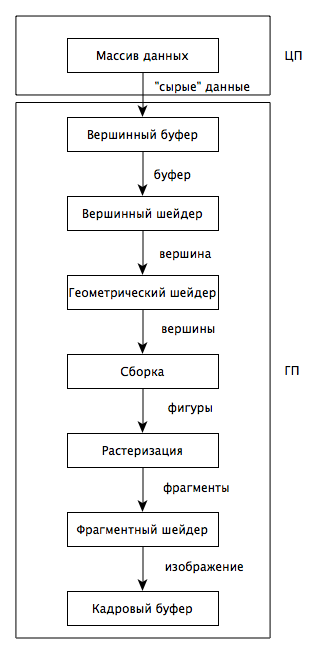
\includegraphics[scale=1.0]{Figures/gpu_pipeline}
\end{center}
\caption{Программируемый графический конвейер}
\label{fig:gpu_pipeline}
\end{figure}


\subsection{Язык шейдеров}

WebGL основан на стандарте OpenGL ES 2.0 \cite{khr11}, который поддерживает только программируемый графический
конвейер. Язык программирования, используемый для написания шейдеров, называется GLSL (OpenGL
Shading Language).

Поддерживаемые в данном стандарте типы шейдеров:

\begin{enumerate}
  \item Вершинные шейдеры. На входе: вершина фигуры. На выходе: преобразованное положение
    вершины. Результат вычислений записывается в специальную переменную gl\textunderscore{}Position.
  \item Фрагментные шейдеры. На входе: координаты на экране и данные, переданные из вершинного 
    шейдера. На выходе: цвет пикселя. Результат записывается в переменную gl\textunderscore{}FragColor.
\end{enumerate}

Когда вершинные и фрагментные шейдеры скомпилированы, они связываются в шейдерную программу.
В каждой программе может содержаться только один вершинный шейдер.

Доступность данных передаваемых внутри программ зависят от того, где они были инициализированы
и строго определяется какие операции могут на них выполнятся. В спецификации GLSL ES 1.0 
существует пять различных модификаторов типов:

\begin{itemize}
  \item Локальные переменные (по умолчанию без ключевого слова)
  \item Константы (ключевое слово const). Значения данного типа формируются во время компиляции и их не
    разрешено изменять при работе программы.
  \item Аттрибуты (ключевое слово attribute). Загружаются на видеокарту из центрального процессора во время передачи массива данных. Видимы в 
    вершинных шейдерах. Значения данного типа так же доступны в режиме только на чтение.
  \item Одинаковые для всех шейдеров (ключевое слово uniform). Передаются с ЦП во время 
    использования программы. Доступны как в вершинных, так и в фрагментных.
  \item Последний модификатор формирует связь между вершинным и фрагментным шейдером. Первый
    формирует какое-то значение для каждой вершины и передает его в вершинную программу.
    Ключевое слово varying.
\end{itemize}

\subsection{Кадровые буферы}

Кадровым буфером называется область памяти для кратковременного хранения данных перед отправкой
на устройство вывода. Данный буфер содержит полную информацию о цветах (значениях) кадра.

Значения кадрового буфера формируется на выходе фрагментного шейдера. Это значит что их можно 
использовать как промежуточное хранилище данных при выполнении алгоритмов. Этап формирования 
конечного изображения через множество программ называются проходом (pass). Содержимое буферов 
можно считывать по известным координатам. Получаемые данные носят название тексел (текстурный 
пиксел). В данном подходе данные остаются непосредственно на видеокарте. Уходит необходимость
постоянно передавать данные на ЦП и обратно, что значительно увеличивает производительность.

Тип данных кадровых буферов определяется стандартом. Выход фрагментных шейдеров представлен в 
GLSL как четырехмерный вектор типа float (числа с плавающей точкой). Передача в другую программу
осуществляется через текстурные блоки. В спецификации WebGL по-умолчанию при связке текстуры
и кадрого буфера доступен только формат byte (неотрицательное число от 0 до 255) \cite{khr11}. 
Это значит что при вычислениях могут быть значительные потери при дискретизации данных. При помощи
расширения OES\textunderscore{}texture\textunderscore{}float можно включить поддержку передачи 
данных типа float.
 % 4 -> 5?? (pictures)
  \newpage
\section{Реализация}

\subsection{Технологии и библиотеки}

Как говорилось ранее, проект реализован под веб-платформу. Для разработки используются следующие технологии:

\begin{itemize}
  \item HTML5 -- язык разметки, используемый для построения структуры и представления веб-страниц. 
    Это пятая версия языка, которая добавляет поддержку тэга \textless{}canvas\textgreater{}, 
    который позволяет скриптовому попиксельному отображению изображений через различные контексты. 
    На момент написания работы, доступно два основных контекста: 2d и webgl.

    2D был первым реализованным типом контекста. Он реализован как абстрактный автомат (схоже 
    с OpenGL) и может быть использован для высокопроизводительной визуализации двухмерных объектов, 
    таких как линии, прямоугольники, кривые, bitmap-изображения и т.д.

    Следующий тип контекста позволил разработчикам создавать высокопроизводительные 3D изображения 
    без использования сторонних плагинов и расширений. Это значит что пользователям не требуется 
    устанавливать дополнительное ПО (например, Adobe Flash Player или Java VM) для просмотра.

  \item Javascript -- динамичный язык программирования. Используется для взаимодействия с 
    пользователями, контроля браузером и асинхронной загрузки ресурсов.

  \item Coffeescript -- язык программирования, который транслируется в javascript. Добавляет 
    синтаксический сахар для повышения краткости и читаемости кода. Например, классы 
    (из объектно-ориентированного программирования), которые имеют четкую и понятную структуру.

  \item WebGL -- спецификация интерфейса для создания динамичных 2D и 3D сцен без использования 
    сторонних плагинов. Создан и поддерживается организацией Khronos Group, на данный момент, 
    разрабатывающей спецификацию OpenGL. WebGL служит связкой между высокоуровневым языком 
    JavaScript и низкоуровневыми операциями на графических процессорах.

  \item GLSL (OpenGL Shading Language) -- язык высокого уровня для программирования шейдеров. 
    Основным преимуществом GLSL является переносимость между платформами и ОС. Т.е. алгоритмы, 
    описанные в рамках данной работы, могут быть перенесены на другие платформы без изменения 
    кода программы.
\end{itemize}

Для упрощения разработки используется Zepto.js. Zepto.js -- библиотека для расширения функционала 
javascript. В частности реализует работу с AJAX запросами, которые используются для загрузки 
ресурсов. Является минималистичным аналогом jQuery, который также может являться альтернативой.

Основным преимуществом данного подхода к реализации является платформонезвисиммость и быстрота разработки.

\subsection{Общая архитектура}
\subsection{Описание алгоритмов}
\subsubsection{Сортировка}
\subsubsection{Поиск ближайших}
\subsubsection{Кластеризация}
\subsubsection{SPH}
 % 7
  \newpage
\section{Тестирование производительности}

Все тесты проводились на демонстрационном примере с различной конфигурацией
симуляции. Основной характеристикой производительности является количество 
кадров в секунду, генерируемых визуализацией.

Для вычисления количества кадров в секунду используются функции стандартной 
библиотеки javascript. Данные снимаются по минимальным значениям показателей.
Для чистоты эксперимента сравнения проводились на разных компьютерах. \\

Конфигурация первого компьютера:

\begin{itemize}
  \item Видеокарта -- Intel HD 4000;
  \item Процессор -- Intel Core i5;
  \item Объем ОЗУ -- 4 гб;
\end{itemize}

Результаты вычислений с различными типами визуализации приведены 
в таблицах \ref{tab:fst:simple}. По горизонтали изменяется количество частиц.
По вертикали тип визуализации.

\begin{table}[H]
  \caption{\label{tab:fst:simple}Комп. №1. Зависимость от типа визуализации}
  \begin{center}
    \begin{tabular}{|c|c|c|c|c|c|}
      \hline
      Тип визуализации & 100 ч. & 1000 ч. & 5000 ч. & 10000 ч. & 100000 ч. \\
      \hline
      Облако точек & 320 & 175 & 97 & 40 & 24 \\
      Направленные векторы & 320 & 170 & 95 & 39 & 23 \\
      \hline
    \end{tabular}
  \end{center}
\end{table}

Одним из параметров, который существенно влияет на скорость визуализации -- это
радиус взаимодействия частиц. Чем он больше, тем большее количество частиц необходимо
обработать. Размер пространства $150\times150$. Радиус указывается в измерениях
виртуального пространства. Результаты тестирования приведены в таблице \ref{tab:fst:radius}.

\begin{table}[H]
  \caption{\label{tab:fst:radius}Комп. №1. Зависимость от радиуса взаимодействия}
  \begin{center}
    \begin{tabular}{|c|c|c|c|c|c|}
      \hline
      Радиус & 100 ч. & 1000 ч. & 5000 ч. & 10000 ч. & 100000 ч. \\
      \hline
      5 & 320 & 175 & 97 & 40 & 24 \\
      10 & 250 & 120 & 84 & 37 & 22 \\
      50 & 100 & 90 & 43 & 20 & 8 \\
      \hline
    \end{tabular}
  \end{center}
\end{table}

Для демонстрации производительности алгоритма поиска ближайших, проведены
тесты с полным перебором. Результаты приведены в таблице \ref{tab:fst:algorithm}.

\begin{table}[H]
  \caption{\label{tab:fst:algorithm}Комп. №1. Зависимость от алгоритма поиска ближайших частиц}
  \begin{center}
    \begin{tabular}{|c|c|c|c|c|c|}
      \hline
      Алгоритм & 100 ч. & 1000 ч. & 5000 ч. & 10000 ч. & 100000 ч. \\
      \hline
      Использование сетки & 320 & 175 & 97 & 40 & 24 \\
      Полный перебор & 343 & 170 & 70 & 20 & 2 \\
      \hline
    \end{tabular}
  \end{center}
\end{table}

В целях демонстрации, так же разработан просчет визуализации на центральном процессоре.
При этом время, затраченное на отображение, не учитывается. Результаты тестирования 
приведены в таблице \ref{tab:fst:cpu}.  \\

\begin{table}[H] 
  \caption{\label{tab:fst:cpu}Комп. №1. Зависимость от типа процессора} 
  \begin{center} 
    \begin{tabular}{|c|c|c|c|c|c|} 
      \hline
      Тип процессора & 100 ч. & 1000 ч. & 5000 ч. & 10000 ч. & 100000 ч. \\
      \hline
      Графический & 320 & 175 & 97 & 40 & 24 \\
      Центральный & 140 & 100 & 30 & 7 & $\approx{}0.3$ \\
      \hline
    \end{tabular} 
  \end{center} 
\end{table} 

Конфигурация второго компьютера:

\begin{itemize} 
  \item Видеокарта -- Nvidia GeForce 640;
  \item Процессор -- Intel Core i7;
  \item Объем ОЗУ -- 8 гб;
\end{itemize} 

Для второго компьютера проведены те же тесты. Результаты приведены в таблицах
\ref{tab:snd:simple}, \ref{tab:snd:radius}, \ref{tab:snd:algorithm}, \ref{tab:snd:cpu}.

\begin{table}[H] 
  \caption{\label{tab:snd:simple}Комп. №2. Зависимость от типа визуализации} 
  \begin{center}
    \begin{tabular}{|c|c|c|c|c|c|}
      \hline
      Тип визуализации & 100 ч. & 1000 ч. & 5000 ч. & 10000 ч. & 100000 ч. \\
      \hline
      Облако точек & 398 & 315 & 150 & 64 & 47 \\
      Направленные векторы & 399 & 310 & 152 & 63 & 46 \\
      \hline
    \end{tabular}
  \end{center}
\end{table}

\begin{table}[H]
  \caption{\label{tab:snd:radius}Комп. №2. Зависимость от радиуса взаимодействия}
  \begin{center}
    \begin{tabular}{|c|c|c|c|c|c|}
      \hline
      Радиус & 100 ч. & 1000 ч. & 5000 ч. & 10000 ч. & 100000 ч. \\
      \hline
      5 & 398 & 315 & 150 & 64 & 47 \\
      10 & 330 & 205 & 130 & 37 & 22 \\
      50 & 340 & 110 & 78 & 20 & 11 \\
      \hline
    \end{tabular}
  \end{center}
\end{table}

\begin{table}[H]
  \caption{\label{tab:snd:algorithm}Комп. №3. Зависимость от алгоритма поиска ближайших частиц}
  \begin{center}
    \begin{tabular}{|c|c|c|c|c|c|}
      \hline
      Алгоритм & 100 ч. & 1000 ч. & 5000 ч. & 10000 ч. & 100000 ч. \\
      \hline
      Использование сетки & 398 & 315 & 150 & 64 & 47 \\
      Полный перебор & 324 & 203 & 121 & 70 & 8 \\
      \hline
    \end{tabular}
  \end{center}
\end{table}

\begin{table}[H]
  \caption{\label{tab:snd:cpu}Комп. №2. Зависимость от типы процессора}
  \begin{center}
    \begin{tabular}{|c|c|c|c|c|c|}
      \hline
      Тип процессора & 100 ч. & 1000 ч. & 5000 ч. & 10000 ч. & 100000 ч. \\
      \hline
      Графический & 398 & 315 & 150 & 64 & 47 \\
      Центральный & 153 & 102 & 31 & 7 & $\approx{}0.4$ \\
      \hline
    \end{tabular}
  \end{center}
\end{table}


% написать как проводились вычисления fps
% различная визуализация
% n^2 и поиск ближайших
% сравнение по количеству частиц
% сравнение на разных gpu
% сравнение cpu и gpu

  \newpage
\section{Руководство пользователя}

Чтобы использовать инструмент, необходимо подключить внешний 
скрипт avr.js при помощи тэга SCRIPT.

%\begin{verbatim}
  %<script type='text/javascript' src='avr.js'></script>
%\end{verbatim}

Для инициализации используется конструктор класса AVR.Context. 
Первым параметром которому передается объект типа CANVAS.

%\begin{verbatim}
  %var avr = new AVR.Context(document.getElementById('display'));
%\end{verbatim}

Для создания визуализации используется метод loadPrograms. Он
позволяет загрузить нужные шейдеры и передать константы. Каждый
из шейдеров автоматически проходит предварительную обработку.
При необходимости в консоль браузера выведется ошибка компиляции.

%\begin{verbatim}
  %avr.loadPrograms({
    %// описание и ссылки на нужные программы
  %}, {
    %// константы
  %}, function(prog) {
    %// код визуализации
  %});
%\end{verbatim}

По-умолчанию для каждой шейдерной программы необходимо указать
vertexUrl и fragmentUrl для вершинного и фрагментного шейдеров соответственно.
Если фрагментный шейдер предполагается использовать для просчета частиц,
ссылку на вершинный шейдер можно опустить.

%\begin{verbatim}
  %avr.loadPrograms({
    %// ...
    %genGridCells : "shaders/gen_grid_cells.glsl",
    %genAccessor  : "shaders/gen_accessor.glsl",
    %bitonicSort  : "shaders/bitonic.glsl",
    %// ..
   
    %axes: {
      %vertexUrl: "shaders/axes.vertex.glsl",
      %fragmentUrl: "shaders/axes.fragment.glsl",
    %}
  %}, { ...
%\end{verbatim}

После загрузки, программы будут доступны в функции обратного вызова.

Чтобы создать конвейер для обработки частиц можно либо вручную писать
использование программ с помощью метода use, либо использовать встроенный
компонент AVR.Chain. Создать цепь можно с помощью метода createChain.

Для того чтобы исполнить программу и вывести содержимое на экран нужно
вызывать метод pass, первым параметром к которому будет программа типа
AVR.Program.

%\begin{verbatim}
  %var c = avr.createChain();
  %c.pass(prog.helloWorld);
%\end{verbatim}

В данном случае начальными данными для вершинного шейдера будут 4
вершины, расположенные в углах экрана (от -1 до 1). Размер кадрового
буфера определяется размером элемента.

Для создания фрагментного буфера в цепи необходимо использовать метод
framebuffer. Первый параметр -- название буфер, второй -- информация о 
фрагментном буфере: размер (size), формат (format), тип (type), начальные
данные (data). Для создания двойного буфера используется метод doubleFramebuffer.
Параметры те же.

%\begin{verbatim}
  %c.framebuffer('reader', { size: size });
  %c.doubleFramebuffer('grid', { size: size });
  %c.doubleFramebuffer('particles', { size: size });
%\end{verbatim}

Чтобы указать в какой кадровый буфер записать результат программы, нужно 
указать селектор вторым параметром в методе pass.

%\begin{verbatim}
  %c.pass(p.fill, 'back particles');
  %c.pass(p.zero, 'back velocities');
  %c.pass(p.zero, 'auto densities');
  %c.pass(p.zero, 'auto pressures');
%\end{verbatim}

Для того, чтобы передать содержимое других буферов в программу третьим
параметром в pass указывается объект где ключами являются названия uniform
переменных, а значениями селектор кадрового буфера.

%\begin{verbatim}
  %c.pass(p.position, 'front particles', {
    %back: 'back particles',
    %velocities: 'front velocities'
  %});
%\end{verbatim}

Для более детальной настройки данного этапа вычислений можно использовать
функцию обратного вызова в методе pass. Первый параметр которой -- объект
содержащий кадровый буфер и программу типов AVR.Framebuffer и AVR.Program.

%\begin{verbatim}
  %c.pass(p.velocity, 'front velocities', {
    %back: 'back velocities',
    %particles: 'back particles',
    %pressures: 'auto pressures',
    %viscosity: 'auto viscosity'
  %}, function(prog) {
    %prog.sendFloat('wallDispl', wallDispl)
  %});
%\end{verbatim}

Для сортировки данных в кадровом буфере используется алгоритмом
битонической сортировки, необходимо использовать метод bitonicSort,
первым параметром которого является название двойного кадрового буфера.
Сортировка происходит по четвертой координате $w$.

%\begin{verbatim}
  %c.bitonicSort('grid');
%\end{verbatim}

Для того чтобы визуализировать результат вычислений, необходимо создать
экземпляр класса AVR.Visual при помощи метода createVisual. Затем
при помощи метода visualize создавать визуальное представление.
Первым параметром в visualize является тип визуализации. Вторым параметром
передается объект для конфигурации визуального представления.

Реализованы следующие типы визуального представления:

\begin{itemize}
  \item AVR.Axes -- рисует оси координат;
  \item AVR.Points -- изобразить в виде точек. По ключу particles
    указывается кадровый буфер из которого будут браться координаты частиц.
    По ключу colors указывается буфер для получения цветов каждой из частиц;
  \item AVR.Vectors -- изобразить в виде векторов. Ключ particles
    указывает кадровый буфер для координат частиц. Ключ colors
    принимает массив из двух элементов с цветами начала и конца вектора. Ключ
    vectors указывает на буфер векторов. Ключ scale содержит число масштаба
    векторов.
\end{itemize}

Для очистки экрана используется метод clear. Перед генерацией следующего
кадра вызывается метод swapBuffers, который меняет местами двойные буферы.

%\begin{verbatim}
  %avr.clear();

  %vis.visualize(AVR.Axes);

  %vis.visualize(AVR.Particles, {
    %positions: c.getBuffer('front particles')
  %});

  %vis.visualize(AVR.Vectors, {
    %positions: c.getBuffer('front particles'),
    %vectors: c.getBuffer('front velocities'),
    %scale: 7
  %});

  %c.swapBuffers();
%\end{verbatim}

Для того чтобы использовать константы в шейдерах используются синтаксис
\$названиеКонстанты.

%\begin{verbatim}
  %vec2 cursor = floor(vec2($sizex, $sizey) / 2.);
%\end{verbatim}

Чтобы исключить дублирование кода в шейдерах, реализовано включение
кода одного из шейдеров в код текущего при помощи директивы. При этом
шейдеры загружаются один раз и включаются в месте написания директивы.

%\begin{verbatim}
  %attribute vec3 vertex;
  %uniform sampler2D positions;

  %$include "shaders/transform.glsl"
 
  %void main() {
    %// ...
%\end{verbatim}

Для создания перспективы и работы с пользовательским вводом
реализованы основные функции в шейдере ``shader/transform.glsl''.

%\begin{verbatim}
  %vec4 perspective(vec3 src); // создает перспективу для точки
  %bool mouseTouch(vec3 part); // возвращает true, если данная 
                                 %частица попала в радиус нажатия

  %vec3 rotation; // содержит текущие углы вращения
  %vec2 mouse; // содержит текущую координату мыши в мировых
                 %координатах (от -1 до 1)
%\end{verbatim}

  \newpage

\section{ВНЕДРЕНИЕ} % 3

Физика большого количества частиц отлично подходит для симуляции множества
природных явлений. Поведение воды, горение огня, физика ткани и т.д.
Находится применение в астрофизике, химии и биологии. Кроме того,
данный подход к вычислениям подходит не только для визуализации, но 
и для вычислений введенных пользователем данных. Например, для кластеризации 
поисковой выдачи в географических информационных системах.

Благодаря выбранной платформе, задача донести информацию до конечного пользователя
значительно упрощается. Нет необходимости устанавливать дополнительные плагины
и расширения для веб-браузера. Упрощается внедрение в уже существующие системы, 
так как большинство обучающих и экспертных систем используют веб-интерфейс.

\subsection{Учебные курсы}

Все большую популярность набирают системы онлайн-образования. К ним можно
отнести такие проекты, как Coursera \footnote{http://coursera.org}, mooc.org \footnote{http://mooc.org}
разрабатываемый компанией Google. Данные системы образования распространяются бесплатно 
и работают как веб-приложения.

Так же подобные визуальные представления могут использоваться при публикации работ студентов 
и ученых на сайтах высших учебных заведений и исследовательских центров.

\subsection{Визуальные представления в экспертных системах}

Разрабатываемое решение может использоваться для создания визуальных представлений
в экспертных системах, предназначенных для диагностики, мониторинга и проектирования
в сложных процессах и механизмах. Полученные визуализации помогут максимально наглядно
донести информацию до пользователя.

\subsection{Игровая индустрия}

Существует несколько примеров игр, которые используют вычислительный метод, описанный 
в документе для создания игрового процесса. Это значит что разработанный инструмент
подходит для создания браузерных HTML5 игр.

Последние версии мобильных браузеров уже добавили поддержку включения WebGL в
экспериментальном режиме. Это значит что на мобильных устройствах так же можно будет
использовать подобный подход для создания визуальных эффектов.

  \newpage
\section{Заключение}

 
  \newpage

  %\catcode`"\active\def"{\relax}
  \renewcommand\refname{Библиографический список}
  \bibliographystyle{gost780s}
  \begin{thebibliography}{}
    \bibitem{webcl10} Khronos Releases WebCL 1.0 Specification -- \url{https://www.khronos.org/news/press/khronos-releases-webcl-1.0-specification}.
    \bibitem{raytracing02} Timothy, J.P. Ray tracing on programmable graphics hardware / T.J. Purcell, I. Buck, W.R. Mark, P. Hanrahan // ACM Transactions on Graphics (TOG). -- 2002. -- V. 21, №3. -- P. 703-712.
    \bibitem{gpu} Fatahalian, K. A closer look at GPUs / K. Fatahalian, M. Houston // Communications of the ACM. -- 2008. -- V. 51, №10. -- P. 50-57.
    \bibitem{hgpuw} Luebke, D. How GPUs Work / D. Luebke, G. Humphreys // IEEE Computer. -- 2007. -- V. 40, №2. -- P. 96-100.
    \bibitem{khr11} WebGL Specification -- \url{http://www.khronos.org/registry/webgl/specs/1.0/}.
    \bibitem{khr09} The OpenGL ES Shading Language \url{http://www.khronos.org/registry/gles/specs/2.0/GLSL\textunderscore ES\textunderscore Specification\textunderscore 1.0.17.pdf}.
    \bibitem{glsl} Rost, R.J. OpenGL Shading Language / R.J. Rost. -- Addison-Wesley Professional, 2006. -- 800 p.
    \bibitem{rtrender} Akenine-Möller, T. Real Time Rendering / T. Akenine-Möller, E. Haines, N. Hoffman. -- A K Peters/CRC Press, 2008. -- 1045 p.
    \bibitem{sphHarada} Harada, T. Smoothed Particle Hydrodynamics on GPUs / T. Harada, S. Koshizuka, and Y. Kawaguchi. -- 2007. -- 8 p.
      In Proc. of Computer Graphics International, pp. 63–70. Geneva: Computer Graphics Society, 2007.
    \bibitem{sphMon92} Monaghan, J.J. Smoothed Particle Hydrodynamics / J.J. Monaghan // Annual Review of Astronomy and Astrophysics. -- 1992. -- V. 30. -- P. 543–574.
    \bibitem{neisearch} Bayraktar, S. GPU-Based Neighbor-Search Algorithm for Particle Simulations / S. Bayraktar, U. Gudukbay, B. Ozguç // J. Graphics Tools. -- 2009. -- V. 14. -- P. 31-42.
  \end{thebibliography}
\end{document}
